\chapter{Numeri Complessi}
\section{Definizione}
Viene definito unità immaginaria $i$ quel numero per cui $i^2 = -1$.
L'insieme dei numeri complessi si definisce quindi come:\\
\begin{equation}
\mathbb{C} = \{z = x + iy;\ x,y \in \mathbb{R}\}
\end{equation}\\
La forma algebrica di un numero complesso $z$ viene definita come:
\[
z = \overbrace{
	\underbrace{x}_\text{parte reale} + i
	\underbrace{y}_\text{parte immaginaria}
}^\text{numero complesso}
\]
\subsubsection{Osservazione}
$z \in \mathbb{C}$ è reale ($z \in \mathbb{R}$) $\iff Imz = 0$

\section{Piano di Gauss}
Il piano di Gauss è un piano $\mathbb{R}^2$ ove l'asse delle ascisse è $Rez$ e l'asse delle ordinate $Imz$. Ogni numero complesso $z$ è quindi rappresentabile come un punto sul piano di Gauss.\\
\begin{figure}[htbp]
	\centering
	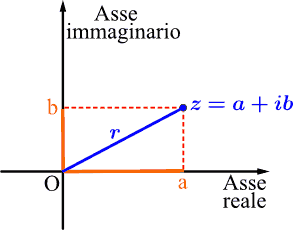
\includegraphics[width=0.3\textwidth]{images/piano_gauss.png}
\end{figure}

\section{Alcune operazioni coi numeri comlessi}
Avendo $z_1,z_2 \in \mathbb{C}$:

\subsection{Somma}
\begin{equation}
z_1+z_2 = x_1+x_2+i(y_1+y_2)
\end{equation}\\
In particolare:\\
$Re(z_1+z_2) = x_1+x_2$\\
$Im(z_1+z_2) = y_1+y_2$
\subsection{Prodotto}
\begin{equation}
z_1z_2 = x_1x_2-y_1y_2+i(x_1y_2+ x_2y_1)
\end{equation}\\
In particolare:\\
$Re(z_1z_2) = x_1x_2-y_1y_2$\\
$Im(z_1z_2) = x_1y_2 + x_2y_1$
\subsection{Modulo}
Avendo $z = x+iy \in \mathbb{C}$, si definisce il modulo di $z$ come:\\
\begin{equation}
|z| = \sqrt{x^2+y^2} \in \mathbb{R}
\end{equation}\\
Nel piano di Gauss, $|z|$ viene rappresentato come la distanza dal punto $z$ all'origine.

\section{Coniugato di z}
Con $z = x+iy \in \mathbb{C}$, si definisce il coniugato di $z$ come:
\begin{equation}
	\bar{z} = x-iy
\end{equation}

\section{Numeri complessi notevoli}
\subsubsection{Elemento neutro somma}
$0\ +\ i0$
\subsubsection{Elemento opposto somma}
$-x\ -\ iy$
\subsubsection{Elemento neutro prodotto}
$1\ +\ i0$
\subsubsection{Elemento reciproco prodotto}
\begin{Large}
$\frac{1}{z}=\frac{1}{x+iy}=\frac{x-iy}{x^2+y^2}$
\end{Large}


\subsubsection{Osservazioni}
Avendo $z_1,z_2 \in \mathbb{C}$, si può dimostrare:\\
\begin{equation}
\begin{gathered}
\overline{1+z_2} = \overline{z_1}+\overline{z_2}\\
\overline{z_1z_2} = \overline{z_1}\overline{z_2}\\
|\bar{z}| = |z|\\
z\bar{z}=|z|^2\\
\frac{1}{z} = \frac{\bar{z}}{|z|^2}
\end{gathered}
\end{equation}

\section{Rappresentazione trigonometrica}
Un numero complesso $z$ può inoltre essere definito come un vettore che ha per origine l'origine del piano di Gauss, come modulo il modulo di $z$ e come direzione un angolo $\theta$:\\
\begin{equation}
\begin{gathered}
z=r(cos(\theta)+isen(\theta)) =\\
r(cos(\theta+2k\pi)+isen(\theta+2k\pi)) \forall k \in \mathbb{Z}
\end{gathered}
\end{equation}

\begin{figure}[htbp]
	\centering
	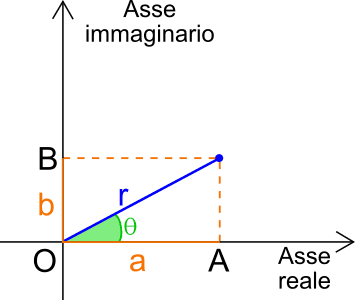
\includegraphics[width=0.3\textwidth]{images/piano_gauss_trigonometria.png}
\end{figure}

In particolare:
\begin{enumerate}
	\item [i.] $r = |z| \geq 0$, in quanto il modulo di un numero complesso è per definizione positivo
	\item [ii.] $\theta$ è detto \textbf{argomento} di $z$
\end{enumerate}

\section{Operazioni con rappresentazione trigonometrica}
\subsection{Prodotto}
Con $z_1,z_2 \in \mathbb{C}$; definiamo $\theta_1 = argz_1,\ \theta_2=argz_2$:

\begin{equation}
z_1z_2=|z_1||z_2|(cos(\theta_1+\theta_2)+isen(\theta_1+\theta_2))
\end{equation}

\subsubsection{Dimostrazione}
\begin{equation*}
\begin{gathered}
z_1z_2=|z_1|(cos(\theta_1)+isen(\theta_1)) * |z_2|(cos(\theta_2)+isen(\theta_2)) =\\
|z_1||z_2|(cos(\theta_1)cos(\theta_2) + i^2sen(\theta_1)sen(\theta_2) + icos(\theta_1)sen(\theta_2) + isen(\theta_1)cos(\theta_2)) =\\
|z_1||z_2|((cos(\theta_1)cos(\theta_2)-sen(\theta_1)sen(\theta_2)) + i(cos(\theta_1)sen(\theta_2) + sen(\theta_1)cos(\theta_2))) =\\
z_1z_2=|z_1||z_2|(cos(\theta_1+\theta_2)+isen(\theta_1+\theta_2))
\end{gathered}
\end{equation*}

\subsection{Potenza (formula di De Moivre)}
Avendo $z \in \mathbb{C}$:\\
\begin{equation}
z^n = |z|^n(cos(n\theta)+isen(n\theta))
\end{equation}
\subsection{Radici n-esime}
$w,z \in \mathbb{C}$\; $n \in \mathbb{N}$\\
Se $n>1$, un numero $z$ è radice n-esima di $w \iff z^n=w$\\
Sia $w \in \mathbb{C}, n \in \mathbb{N}, n>1, w=|w|(cos(\theta)+isen(\theta)$:\\
\begin{enumerate}
\item[i.] Se $w=0$ la sola radice di $w$ è $z=0$
\item[ii.] Se $w\neq0$ allora $w$ ha \textbf{n} radici \textbf{distinte} che sono:\\
\begin{equation}
z_k=\sqrt[n]{|w|}(cos(\frac{\theta+2k\pi}{n})+isen(\frac{\theta+2k\pi}{n})),\ k \in \mathbb{N},\ 0\leq k<n
\end{equation}
\end{enumerate}
\subsubsection{Dimostrazione}
\begin{enumerate}
\item[i.]$w=0 \iff |z^n|=0 \iff |z|=0 \iff z=0$
\item[ii.]$z=|z|(cos(t)+isen(t))$; $z^n=w \iff \\
|z|^n(cos(nt)+isen(nt)) = |w|(cos(\theta+2k\pi)+isen(\theta +2k\pi) \iff
\begin{cases}
|z|^n = |w|\\
nt = \theta +2k\pi
\end{cases}$
\end{enumerate}
\subsection{Teorema fondamentale dell'algebra}
L'equazione polinomiale della forma: $a_nz^n + a_{n-1}z^{n-1}+...+a_1z+a_0$, $a_n \neq 0$, $a_i \in \mathbb{C}$ ha esattamente \textbf{n} radici in $\mathbb{C}$

\subsection{Notazione Esponenziale}
Per la formula di Eulero:\\
\begin{equation}
	e^{i\theta} = cos(\theta)+isen(\theta)
\end{equation}
Un numero complesso $z = |z|(cos(\theta)+isen(\theta))$ si può esprimere in notazione esponenziale come:\\
\begin{equation}
z = |z|e^{i\theta}
\end{equation}\\